\chapter{Multivariate Maps}
\label{chap:MultivariateMaps}
\bibentry{mcnabb2019multivariate} \cite{mcnabb2019multivariate} \\
\chapterquote{Statistics are like bikinis. What they reveal is suggestive, but what they conceal is vital.}
{Aaron Levenstein, Business Professor at Baruch College}



\newpage
{\footnotesize \hypersetup{linkcolor=black}
\minitoc}

%-------------------------------------------------------------------------
%\begin{abstract}
\newpage
\topskip0pt
\vspace*{4cm}
\section*{Chapter Abstract}
Maps are one of the most conventional types of visualization used when conveying information to both inexperienced users and advanced analysts. However, the multivariate representation of data on maps is still considered an unsolved problem. We present a multivariate map that uses geo-space to guide the position of  multivariate glyphs and enable users to interact with the map and glyphs, conveying meaningful data at different levels of detail. We develop an algorithm pipeline for this process and demonstrate how the user can adjust the level-of-detail of the resulting imagery. We present a selection of user options to facilitate the exploration process and provide case studies to support how the application can be used. We also compare our placement algorithm with previous geo-spatial glyph placement algorithms. The result is a novel glyph placement solution to support multi-variate maps.
%\end{abstract}  
\clearpage
%-------------------------------------------------------------------------
\section{Introduction and Motivation}
In this chapter, we move toward extending our existing algorithm to support new features, including multivariate data and glyph placement. We also present the robustness of our design using real-time filters and animation.

Maps are useful for conveying information to both inexperienced and advanced users. There are many types of maps designed to present data but the underlying maps often come with other challenges such as the how the areas are segmented. Fairbairn et al.\ suggest scale, level of detail, and multivariate data as common challenges for the representation of geo-spatial data \cite{fairbairn2001representation}.  Ward et al.\ state, \emph{"A problem of choropleth maps is that the most interesting values are often concentrated in densely populated areas with small and barely visible polygons, and less interesting values are spread out over sparsely populated areas with large and visually dominating polygons."} The challenge of perception (\textbf{C1} -- size perceivability) is a fundamental one associated with digital maps. Even when trying to rectify this for a univariate map, few solutions enable opportunities to convey multivariate, high-dimensional data. For example, geo-spatial designs (choropleths, cartograms, symbol maps, etc.) only depict uni-variate, or occasionally, bivariate data. This is a challenge regarding the conveying of multi-variate geospatial data (\textbf{C2} -- multivariate geospatial data). One possibility is glyphs to support multivariate visualization options. However, even if we can present multivariate geospatial data using glyphs, we still run into challenges. If we plot glyphs in their geospatial context, then we risk overlap and over-plotting. In other words, if we place a multivariate glyph at the center of each unit area on a map, the glyphs will either overlap in many cases or be too small to perceive, especially in densely populated areas (see Figure \ref{fig:ccgs}) (\textbf{C3} -- occlusion). Ellis and Dix state \emph{"a glyph representing multiple attributes may need simplifying when reduced in size, resulting in a loss of data"} \cite{ellis2007taxonomy}, suggesting that reducing the size of a scalable multivariate glyph can be problematic (\textbf{C1} -- size perceivability). Another option to address \textbf{\textbf{C3} -- occlusion} is to employ structure-driven glyph placement guided by a Cartesian grid. However this common solution de-couples the glyphs from the original geospatial areas they intend to represent. This is the challenge of geo-spatial glyph-placement (\textbf{C4} -- glyph placement).
In order to address all four challenges, \textbf{C1--C4}, we introduce scale-aware maps, a process of presenting geo-spatial multivariate data based on a desired screen space,  that enables dynamic modification to the level of detail shown using both zooming functions and custom scale options. We integrate this with glyphs to present multivariate data in a geo-spatial context to enable interactive exploration, and facilitate easier comprehension with area context using both smooth transitions and uncertainty indicators. We refer to our work as using glyphs as opposed to symbols guided by the definition from Borgo et al.\ who define glyphs as, \emph{"...an independent visual object that depicts attributes of a data record"} \cite{borgo2013glyph}. Our contributions include:
\begin{figure*}[t]
\centering
%\subfigure[]{
%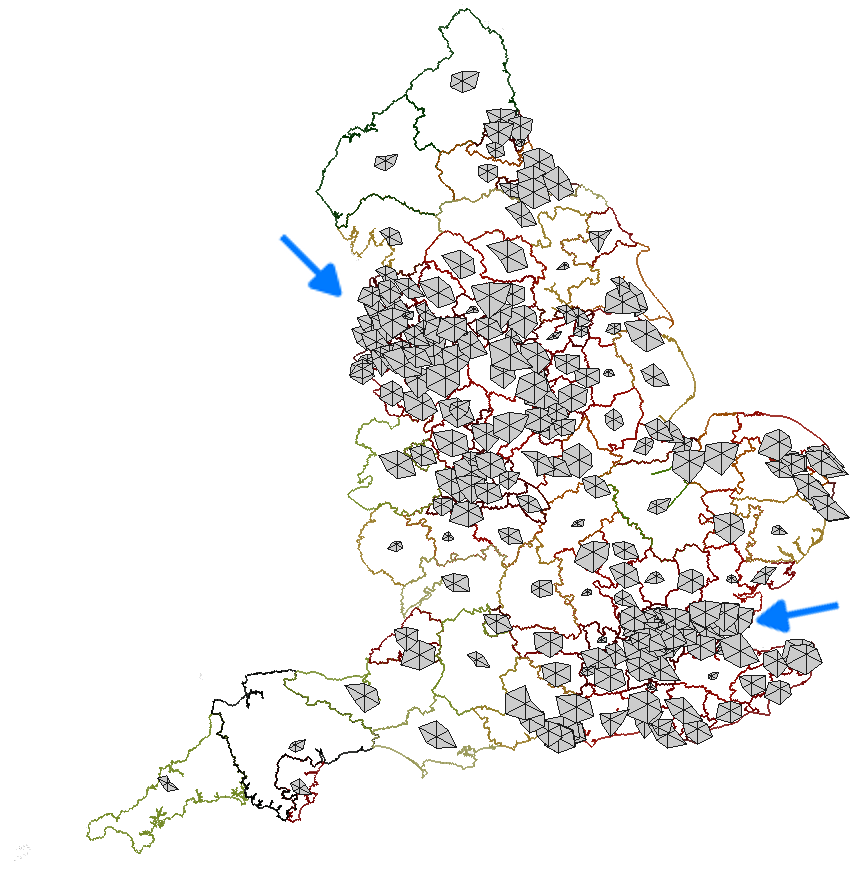
\includegraphics[width=0.4\textwidth]{images/CCGStarDefault.png}}
%\subfigure[]{
%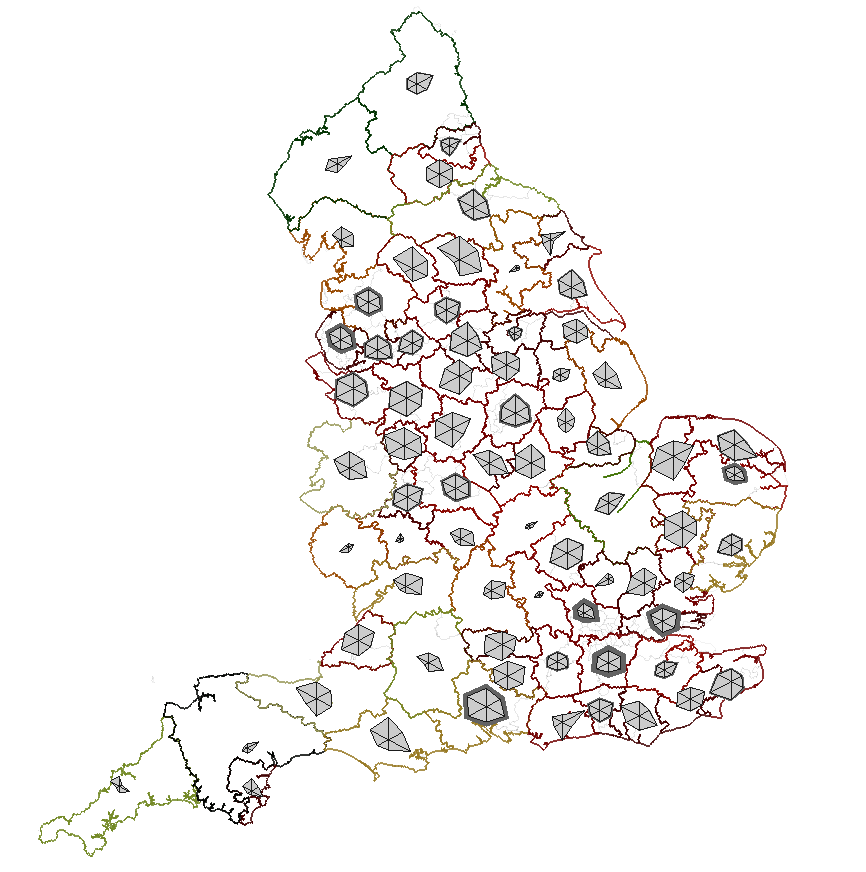
\includegraphics[width=0.4\textwidth]{images/CCGStarBasic.png}}
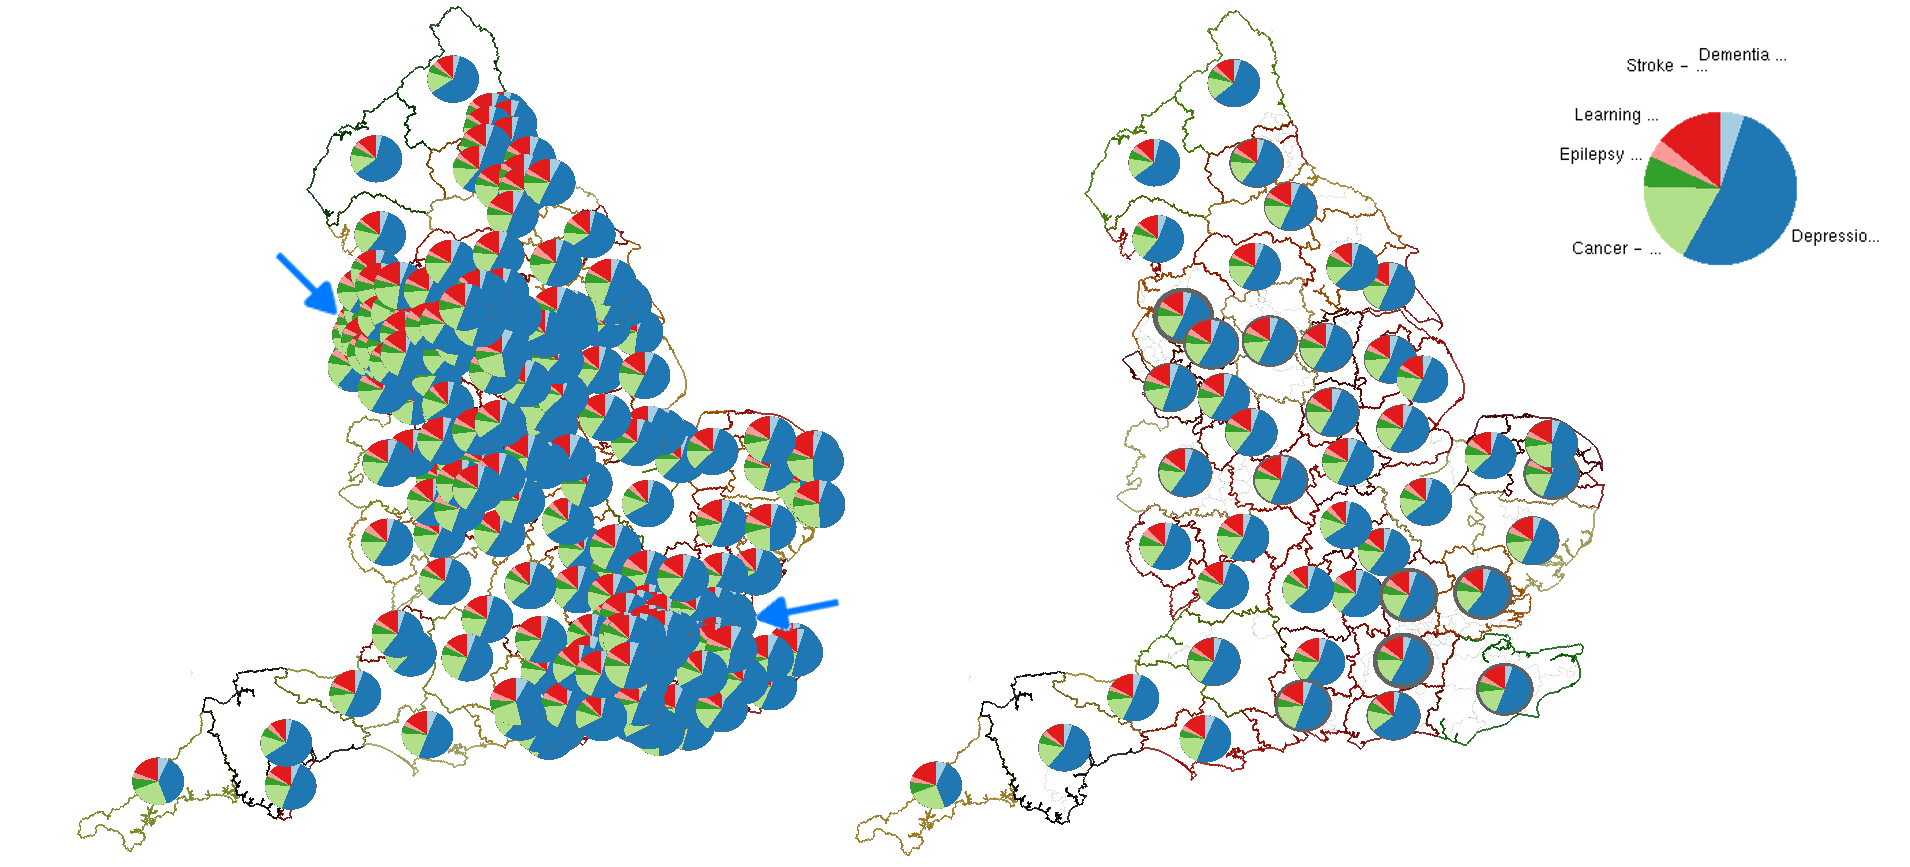
\includegraphics[width=0.95\textwidth]{images/ch5/ccgsetPie2}
\caption{(left) The representation of population health data based on the Clinical Commisioning Groups (CCGs) of England \cite{publicHealthEngland}. Refer to Section \ref{sec:case} for a case study. Glyphs that are simply placed at the centroid of each region are over-plotted and occluded around London, Manchester, and Liverpool (indicated by blue arrows). (right) Our result using level-of-detail scale-aware maps. Even at a small scale for the figure, we can still clearly differentiate each area's glyph.} \label{fig:ccgs}
\end{figure*}
\begin{itemize}[labelindent=0em, labelsep=0.2cm, leftmargin=*]
\item[\textbf{1.}] A multivariate map with scalable glyph rendering and presentation (in the form of scale-aware maps) (\textbf{C1} -- size perceivability, \textbf{C2} -- multivariate geospatial data, \textbf{C4} -- glyph placement).
\item[\textbf{2.}] Dynamic glyphs that support zooming, and user-controlled level of detail. (\textbf{C2} -- multivariate geospatial data, \textbf{C3} -- occlusion, \textbf{C4} -- glyph placement)
\item[\textbf{3.}] Interactive filters to improve analysis and exploration of multivariate data and comparison of geo-spatial areas. (\textbf{C2} -- multivariate geospatial data)
\end{itemize}
In order to do so, we develop solutions that address the four major challenges, \textbf{C1--C4}.

%-------------------------------------------------------------------------

\section{Background}
Our literature review in Chapter \ref{chap:SoS} includes a section of glyph-focused survey papers, as well as geospatial surveys. Borgo et al.\ present a survey of glyph design criteria \cite{borgo2013glyph}. Fuchs et al.\ provide a systematic review of experimental studies on data glyphs \cite{fuchs2016systematic}.
Ward presents a taxonomy of different glyph placement strategies (discussed further in the glyph placement section) \cite{ward2002taxonomy}. We find three survey papers on cartograms \cite{tobler2004thirty, nusrat2015task, nusrat2016state}. We do not consider univariate cartograms within the scope of our work as they distort the boundary geometry of the geo-spatial data, which we avoid in our process.

\textbf{Related Work with a focus on Multivariate Maps:~} Multivariate maps have been used in cartography for over 100 years. For example, Minard depicts a multivariate map using pie charts to present cow consumption across France \cite{minard1858carte}. The pie charts are placed manually.
Kahrl et al.\ present a range of imagery focused on California's water supplies including irrigation applied to crops in the form of dense pixel displays across geo-spatial points \cite{kahrl1978california}. 
Approaches to add more dimensions to choropleths include bivariate color maps \cite{olson1981spectrally, dunn1989dynamic}.
Dorling visualizes local urban changes across Great Britain \cite{dorling1995visualization}. The paper uses multivariate options to review industry distribution, owner-occupied housing, as well as a set of attributes plotted using Chernoff faces as a equal area representation.
Brewer and Campbell present point symbols for representing quantitative data on maps, including bi-variate options \cite{brewer1998beyond}. Although their paper does not focus on placement. Their examples place symbols on a centroid, and show minor occlusion.
Andrienko and Andrienko \cite{andrienko2006exploratory} contains a range of examples of multivariate maps using glyphs for thematic maps, including temporal glyphs, and multivariate pie glyphs for forest data. 
Slocum et al.\ provide a chapter on multivariate maps, describing techniques to consider when displaying bivariate, trivariate, and multivariate data \cite{slocum2009thematic}. 
Slingsby et al.\ capture the geo-spatial context and transform their results into a grid, which is then represented by a treemap where the hierarchy is based on temporal data \cite{slingsby2010treemap}.
 Slingsby et al.\ present a rectangular cartogram showing the postcodes in Great Britain, where postcode district and unit postcodes form the hierarchy \cite{slingsby2010rectangular}. Cartograms distort geo-space, which we avoid using our procedure.
Elmer review symbol consideration for bivariate thematic maps, but do not support more than two variates \cite{elmer2012symbol}. Our algorithm supports an arbitrary number of variants depending on the glyph design.
Kresse and Danko present geographic techniques from basic principles to applications \cite{kresse2012springer}. They present a table of visual variables to represent data, applied to a given map and symbols.

\begin{figure*}
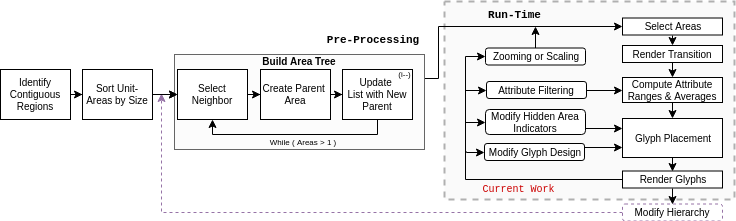
\includegraphics[width=0.9\textwidth]{images/ch5/HorizontalFlow2}
\caption{The flow chart of the procedure. The right square represents what is discussed in the scope of this paper, the pre-processing steps are discussed in Chapter \ref{chap:dcm}.} \label{fig:procedure}
\end{figure*}

Tong et al.\ develop Cartographic Treemaps to explore multivariate medical data provided by Public Health England \cite{tong2017cartographic}. This is extended to time-varying data \cite{tong2017time}. 
Tsorlini et al.\ present a taxonomy of thematic cartography symbols, including multivariate options \cite{tsorlini2017designing}. The symbols are presented as a hierarchy, focusing on the amount of attributes, and arrangement.
Beecham et al.\ visualize trends to explain the UK's vote to leave the European Union. They use a juxtaposed view to presented equal area cartograms for different variants \cite{beecham2018locally}. 
Nusrat et al.\ produce a cartogram that presents bi-variate data using a ring encoding, where the color presents the leading statistic, and the ring thickness presents the value the leading statistic leads by \cite{nusrat2018cartogram}. 


\textbf{ Related Work with a focus on Glyph Placement:~} 
Ward and Lipchak create a software tool for cyclical, temporal multivariate data. Glyphs are placed in an ordered grid structure to enable easy comparison between similar months, or entire years \cite{ward2000visualization}. They also use a radial structure. Our work differs from this work by focusing the glyph placement coupled to geo-spatial areas. 
Ward presents a taxonomy of different glyph placement strategies \cite{ward2002taxonomy}. They introduce  glyph designs that can be used, and 15 glyph placement strategies together with a flow chart of how the glyph placement is driven (data-driven or structure-driven). Our placement strategy is considered geo-spatially data-driven. As the modifications are made before the placement process, it falls into original->derived->data-driven. This is expanded by a subsection in a further Ward survey \cite{ward2008multivariate}.
Andrienko and Andrienko present glyph placement in a selection of ways, for example standard symbol placement for US states and a Cartesian grid to represent forest data over Europe \cite{andrienko2006exploratory}. They discuss the importance of the link between identifying a symbol and the geo-space it represents (on the map) (\textbf{C4} -- glyph placement).
Ropinski and Preim present a taxonomy of usage guidelines for glyph-based medical visualization \cite{ropinski2008taxonomy}. As opposed to Ward's placement taxonomy, they suggest glyphs should be placed based on physical characteristics or anatomical features.
Borgo et al.\ provide a section on glyph placement which extends on both of the previous taxonomy by suggesting user-driven placement \cite{borgo2013glyph}.
Chung et al.\ discuss glyph sorting strategies and present horizontal axis bins, applying it to sport-event analysis glyphs \cite{chung2015glyph}. Our work differs by guiding our glyph placement strategy based on a geospatial, 2D context.

\section{Design Goals and Tasks} \label{sec:tasks}
We derive six mains tasks to motivate our design process. 

\begin{itemize}[labelindent=0em, labelsep=0.1cm, leftmargin=*]
\item[\textbf{T1}]\textbf{-- Overview:} Provide a glyph-based overview of multivariate data on a map free from occlusion (\textbf{C3} -- occlusion).
\item[\textbf{T2}]\textbf{-- Multivariate Map:} Offer a selection of informative multivariate glyphs to compare trends between regions (\textbf{C2} -- multivariate geospatial data).
\item[\textbf{T3}]\textbf{-- Glyph Placement:} Clearly couple encoded glyphs to their geo-spatial contexts (\textbf{C4} -- glyph placement).
\item[\textbf{T4}]\textbf{-- Occlusion} Leverage scale-aware maps to enable exploration of the data at multiple levels of detail (\textbf{C1} -- size perceivability).
\item[\textbf{T5}]\textbf{-- Filtering:} Support the exploration of multivariate geo-spatial data with user options with varying glyph designs and filters (\textbf{C2} -- multivariate geospatial data).
\item[\textbf{T6}]\textbf{-- Fluid Interaction:} To provide smooth and fluid transitions between the different levels of detail for fluid interaction (\textbf{C4} -- glyph placement).
\end{itemize}
\section{Overview}
This section provides the pre-processing steps used to create the scale-aware maps, the run-time process for transitioning between glyph densities, and the options we provide to enhance the exploration of the data. The pre-processing steps are based on previous work in Chapter \ref{chap:dcm}. The purpose of the pre-processing step is to build a dynamic map whose areas are always perceivable, unit areas that are too small (refer to Chapter \ref{chap:userStudy}) are unified until they reach a minimum area threshold set by the user. We build a hierarchical area-based data structure before displaying a dynamic choropleth map.
We separate regions into islands (or land masses) for topological continuity. Once each contiguous region is identified, each unit-area within the same contiguous region is sorted in order of increasing size, since scale is an important part of the algorithm. The area-based hierarchy construction is a recursive algorithm broken down into three sub-routines. In these three steps, we select the optimal neighbor for merging, we identify the shared boundary between the given area and its neighbor, and unify them to create a new area which is then inserted back into the list of areas sorted by size. A flow chart of the procedure is found in Figure \ref{fig:procedure}.

\subsection{Pre-processing}
%\textbf{Order Vertices:}
\textbf{Contiguous Regions:} In order to reduce the complexity of the hierarchy construction, we group unit areas into contiguous regions. If a given land mass or island identifies a neighboring unit-area, we recognize that every other region belonging to the land mass is also linked contiguously. We can then merge the two areas and continue our search. It is important that we do not terminate the search here as our new unit-area may join multiple land masses or islands together. Once this process is complete for each unit-area, we have identified each contiguous region. \\
\textbf{Build Hierarchy:} We use a recursive procedure to create a hierarchical area-based data structure. An area hierarchy is created for each contiguous region, where each area is merged with its closest neighbor identified using a customizable distance metric (refer to Chapter \ref{chap:dcm}). We start with a merge candidate list filled with the sorted unit-areas (for one contiguous region). There are three main sub-routines: (a) neighbor selection, (b) creating the parent area, and (c) updating the merge candidate list. If only a single unit-area remains in the merge candidate list, no further merges can be processed and the procedure terminates. (a) In order to select an appropriate neighbor to join, we use a general and flexible distance metric for amalgamation evaluated between neighboring areas.

We use the closest distance considered as the optimal selection for a neighbor,
$D = w_a.\frac{a}{a_{max}} + w_d.\frac{d}{d_{max}} + w_\alpha.\frac{\alpha}{\alpha_{max}} + w_{b_s}.(1-\frac{b_s}{b_{s_{max}}})$.
The measure consists of four constituents: Smallest area ($a$), euclidean distance between centroids ($d$), value variance ($\alpha$), and shared boundary resolution ($b_s$). We search and identify each common vertex between neighboring areas to identify the shared boundary. We update the sorted area list by removing the two merged areas, and inserting the newly created parent, which may be used as a new merge candidate. This is repeated until only one area remains in each contiguous region.\\
\textbf{Value calculation for unified areas:} The Modifiable Areal Unit Problem (MAUP) \cite{openshaw1984modifiable} is an important aspect to consider when discussing the modification of boundaries or values. We address this by providing the user options to customize calculation of aggregated values as well as the customizable distance metric used to evaluate area merge candidates. The multivariate data is linked to the unit areas during the initial loading of the shape files. Before the area tree is built, the user can select the type of value amalgamation. This enables the user to choose options of sums,  frequencies, and value averages. When amalgamating values using sums, the value can be calculated using aggregation. Qualitative values are calculated using frequencies. For a detailed description of parent value calculation, see Chapter \ref{chap:dcm}.
\subsection{Geospatial Glyph Placement} \label{sec:rendering}
We select visible areas and glyphs based on a minimum area scale requirement (a percentage), $m$ (see Section \ref{sec:scaleAdjust}). When the map is rendered, the tree is traversed using a depth-first search (DFS) to identify which areas are rendered. If an area is larger than $m$ we test two criterion: if the area is a leaf node, or if either the left or right child is smaller than $m$. If either of these true, we render the area. For each area displayed, we create a glyph using the area's centroid to position the glyph. We create a glyph that reflects the given area's multivariate data values (based on the user's selection, see Section \ref{sec:glyphSelect}). As the zoom level of the map changes, different areas may meet $m$ and therefore be presented, creating a dynamic presentation of glyphs. This addresses \textbf{T1 -- Overview} and \textbf{T3 -- Glyph Placement}, by providing a clear overview of the map with no occlusion, and clearly encoded geo-spatial context.

\begin{figure*}
\centering
%\subfloat{
%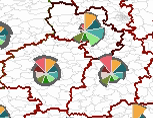
\includegraphics[width=0.18\linewidth]{images/transition/01.png}}
%\subfloat{
%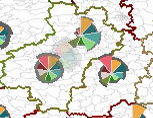
\includegraphics[width=0.18\linewidth]{images/transition/02.png}}
%\subfloat{
%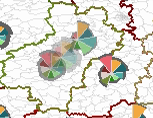
\includegraphics[width=0.18\linewidth]{images/transition/03.png}}
%\subfloat{
%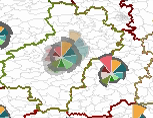
\includegraphics[width=0.18\linewidth]{images/transition/04.png}}
%\subfloat{
%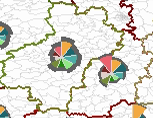
\includegraphics[width=0.18\linewidth]{images/transition/05.png}}
\subfloat{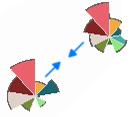
\includegraphics[width=0.12\linewidth]{images/ch5/transition/11}}
\subfloat{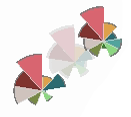
\includegraphics[width=0.12\linewidth]{images/ch5/transition/12}}
\subfloat{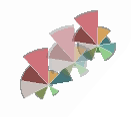
\includegraphics[width=0.12\linewidth]{images/ch5/transition/13}}
\subfloat{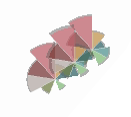
\includegraphics[width=0.12\linewidth]{images/ch5/transition/14}}
\subfloat{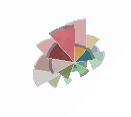
\includegraphics[width=0.12\linewidth]{images/ch5/transition/15}}
\subfloat{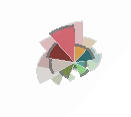
\includegraphics[width=0.12\linewidth]{images/ch5/transition/16}}
\subfloat{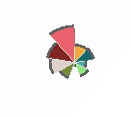
\includegraphics[width=0.12\linewidth]{images/ch5/transition/17}}
\caption{An example of a smooth transition made between two child glyphs that translate towards the new parent node. Both child glyphs decrease in opacity, whilst the new parent glyph increases in opacity. Refer to Section \ref{sec:transitions}.} \label{fig:transitions}
\end{figure*}

\begin{figure}
\centering
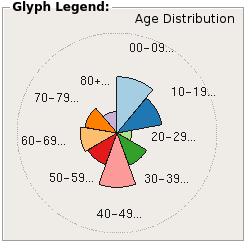
\includegraphics[width=0.55\linewidth]{images/ch5/GlyphLegend2}
\caption{A representation of a glyph legend. The data represents the prevalence of population per age range. The dotted circle represents the full scale of the glyph or the largest value for each dimension. The glyph legend shows the average values over the whole data set. Refer to Section \ref{sec:legend}.} \label{fig:legend}
\end{figure}

\begin{table}[b]
\begin{tabular}{|m{2cm}|m{1.5cm}|m{1.5cm}|m{1.5cm}| >{\centering\arraybackslash}m{1.5cm}|} \hline
&\multicolumn{4}{c|}{Hidden Density Indicators}\\ \cline{2-5}
\multirow{-2}{2cm}{\centering Glyph Design}&\centering Outline &\centering Size &\centering Shadow & Size + Outline\\ \hline &&&&\vspace{-0.3cm}\\
\centering Pie Chart&
\Centerstack{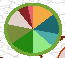
\includegraphics[width=\linewidth]{images/ch5/glyphs/pie1.png}}&
\Centerstack{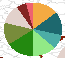
\includegraphics[width=\linewidth]{images/ch5/glyphs/pie2.png}}&
\Centerstack{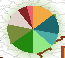
\includegraphics[width=\linewidth]{images/ch5/glyphs/pie3.png}}&
\Centerstack{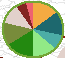
\includegraphics[width=\linewidth]{images/ch5/glyphs/pie4.png}}\\
\centering Polar Area Chart&
\Centerstack{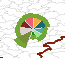
\includegraphics[width=\linewidth]{images/ch5/glyphs/wheel1.png}}&
\Centerstack{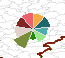
\includegraphics[width=\linewidth]{images/ch5/glyphs/wheel2.png}}&
\Centerstack{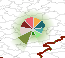
\includegraphics[width=\linewidth]{images/ch5/glyphs/wheel3.png}}&
\Centerstack{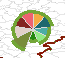
\includegraphics[width=\linewidth]{images/ch5/glyphs/wheel4.png}}\\
\centering Bar Chart&
\Centerstack{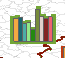
\includegraphics[width=\linewidth]{images/ch5/glyphs/bar1.png}}&
\Centerstack{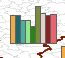
\includegraphics[width=\linewidth]{images/ch5/glyphs/bar2.png}}&
\Centerstack{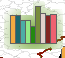
\includegraphics[width=\linewidth]{images/ch5/glyphs/bar3.png}}&
\Centerstack{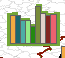
\includegraphics[width=\linewidth]{images/ch5/glyphs/bar4.png}}\\
\centering Star Chart&
\Centerstack{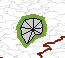
\includegraphics[width=\linewidth]{images/ch5/glyphs/star1.png}}&
\Centerstack{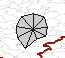
\includegraphics[width=\linewidth]{images/ch5/glyphs/star2.png}}&
\Centerstack{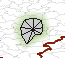
\includegraphics[width=\linewidth]{images/ch5/glyphs/star3.png}}&
\Centerstack{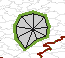
\includegraphics[width=\linewidth]{images/ch5/glyphs/star4.png}}\\ \hline
\end{tabular}
\caption{Previews of the different glyphs, and the hidden density indicators provided in the application. Each glyph represents the same area, reflecting the same hidden indicator values, and attributes. Refer to our third case study, Section \ref{sec:case}, for more details on the values.} \label{tab:glyph}
\end{table}

\subsection{Glyph Selection} \label{sec:glyphSelect}


We provide the user four common glyph design options to represent the data (see Table \ref{tab:glyph}). We chose these four typical options due to their common occurrence in geo-spatial literature \cite{andrienko2006exploratory}. However, the principles we describe can be applied to any multi-dimensional glyph. The user can switch between each glyph design at any point once the hierarchical data structure has been built. These glyph options are:\\
\textbf{Pie Chart:} Pie charts are an easily recognizable and practical design, making it a suitable option to present multivariate data. Pie charts are primarily used to present distribution per geospatial area, where the angle of a segment is mapped to each data dimension proportionally. See Table \ref{tab:glyph}.\\
\textbf{Polar Area Chart:} Originally published by Nightingale \cite{nightingale1858notes}, a polar area chart is another radial plot but with equal segment angles. The radius or each slice corresponds to the values of each dimension, which facilitates comparison between geo-spatial areas. The polar area chart features different names including the wheel, coxcomb, or wing chart. See Table \ref{tab:glyph}. \\
\textbf{Bar Chart:} The bar chart is one of the most visually recognizable visual designs. Values are assigned to bar heights. aligned to the horizontal axis for easy value comparison. See Table \ref{tab:glyph}.\\
\textbf{Star Glyph:} Originally presented by Siegel et al.\cite{siegel1972surgical}, a star glyph presents values using lines originating from the same point, at equal angles. The endpoints connect to form a unique polygon based on the length of each line. See Table \ref{tab:glyph}.\\ This addresses the requirements for \textbf{T2 --Multivariate Maps}. We choose four standard glyph designs as a proof-of-concept. Glyph placement, not glyph design is the focus of this paper. The principles we present can be extended to any multivariate glyph.

\subsection{Adjusting Level-of-Detail with Glyph Density} \label{sec:scaleAdjust}
Adjusting glyph density can be handled in two different ways. First, we give the user a slider which depicts $m$, a minimum area requirement. The parameter $m$ represents a percentage of screen space. This is used as the primary variable for the depth-first search (DFS) discussed in Section \ref{sec:rendering}. We also allow the user to interactively zoom in or out of the map. This changes the visible extents of the map, modifying the screen space covered by each area. These options enable the rendering of perceivable glyphs, meeting the requirements for \textbf{T4 -- Occlusion}.

\begin{figure*}[t]
\centering
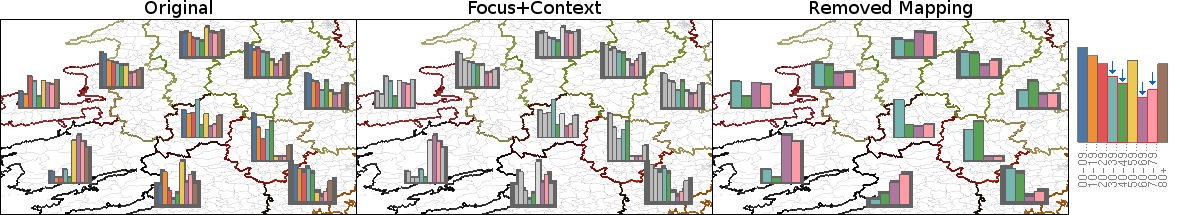
\includegraphics[width=1\textwidth]{images/ch5/f+cv2}
\caption{Our filtering options. The left shows our original image. The center shows our focus+context rendering, which represents the context in greyscale. The right image shows our mapping filter, which redraws the data based on the focus dimensions. The legend indicates the focus dimensions using the blue arrows. Refer to Section \ref{sec:filter}. The Munster area refers to the bottom-left glyph, which is notable for Case Study 3, Section \ref{sec:case03}.} \label{fig:f+c}  \vspace{-0.2cm}
\end{figure*}

\subsection{Smooth Merging and Splitting Transitions} \label{sec:transitions}
In order to increase the fluidity of user interaction and changes to glyph size when zooming or manipulating $m$, we apply smooth transitions to child glyph merging and parent glyph splitting. When the user reduces the number of glyphs by either zooming out of the map or increasing the level of detail, glyphs translate towards the origin of their parent in the hierarchy while the opacity is reduced until it is no longer visible. The parent increases in opacity until it is fully opaque, creating a smooth transition. When adding new glyphs (zooming in or reducing minimum scale), the new child glyphs translate away from their parent and increase in opacity to provide a similar effect. Using this technique, we fulfill the requirement for \textbf{T6 -- Fluid Interaction}. See Figure \ref{fig:transitions}.

\subsection{Dynamic Average Glyph Legend} \label{sec:legend}
We provide a dynamic average glyph legend to present how the multivariate data dimensions of the glyph are encoded. Each variate is given a label, which provides context to the user about what is presented. The data used to present the glyph is made meaningful by visualizing the average value of each dimension. In Figure \ref{fig:legend}, we can see that there seem to be some extreme values for the 80+ and 20--29 range, causing the average per area to be quite small overall.


\subsection{Attribute Filtering} \label{sec:filter}
Our first filter option is to re-calculate the glyph design with only the toggled dimensions. Each data dimension can be toggled using a check-box incorporated directly into the glyph design. This allows the user to focus on or emphasize data dimensions that may reveal trends. We support user filtering using focus+context rendering. We provide a gray-scale option which removes the color from context data dimensions, enabling easier comparison. This aids in the requirements we set forth in \textbf{T5 -- Filtering}. See Figure \ref{fig:f+c}.

\subsection{Unit Area Density Indicators}
We present unit area density indicators that provide a visual queue indicating how hidden unit areas are distributed, and encourage the user to explore the visualization through multiple levels of detail. When two child glyphs merge to form a parent, the child glyphs are then hidden. Our glyph design maps the number of merges to a range of different visual indicators that generally surround the glyph. See Table \ref{tab:glyph}. We offer four options:\\
\textbf{Outline:~} Outline maps the unit area quantity around each glyph to thickness. The thickness of the outline grows as more areas fall underneath a glyph.\\
\textbf{Size:~} Rather than provide an outline, the glyph's overall size increases as the glyph represents more unit areas. This works especially well with pie charts, that emulate a proportional map. \\
\textbf{Size+Outline:~} Size + Outline uses a combination of the two previous options.\\
\textbf{Shadows:~} Rather than an outline with a constant opacity, we enable for the user to choose a gradient, enabling less occlusion in the representation.\\
These unit area density indicators are inspired by the work of Chung et al.\ \cite{chung2015glyph} where the indicator was effective, but used to represent another data dimension (as opposed to the density of a map).
We also give the user an option to represent the indicator mapped to color. The color represents the scale the glyph encodes, as opposed to other visible encodings. This enables the user to gain an understanding of how manipulation of glyph density can affect the map if a transition is made. See Figure \ref{tab:glyph}. This addresses our requirements of \textbf{T4 -- Occlusion}.

\subsection{Interactive User Options}
We provide additional user options to support \textbf{T5 -- Filtering}. We present a range of user options including value range filters, advanced focus+context rendering options, estimated glyph placement, and context administrative areas.\\
\textbf{Data Range Options:} We provide data range filtering to enable customized local and global design options for dimension encoding. On a local range, the user can shift the value range to present the data dimensions based on the values found in the leaf nodes (the original dataset), or clamp the ranges amongst those that are currently being rendered to enable a more accurate data range to compare data dimensions. We also support global range options by enabling the user to depict each variant based on its own range, or by creating a range based on the highest and lowest value of all mapped dimensions.  \\
\textbf{Advanced Filters:} We include two advanced filters to render focus+context for the user. For numerical values, the user can present focus+context based on values higher or lower than the average value per data dimension.\\
\textbf{Color Map:} We provide the user with a variety of color maps, selected from published research papers, including ColorBrewer \cite{brewer2003transition} (Refer to Table \ref{tab:glyph}) and Colorgorical \cite{gramazio2017colorgorical} (Refer to Figure \ref{fig:f+c}).\\
\textbf{Glyph Scaling:} We allow the user to scale the size of the glyph. This enables the user to explore a ratio between the minimum scale and size of glyphs that meets their own data.\\
\textbf{Naive estimated glyph placement:} Using the size of the glyph, we can support the user to make an estimation of the minimum screen space necessary to remove occlusion with the use of a button. This makes it easier to obtain a starting point, in order to decide the design of the map they would like to use.\\
\textbf{Context Administrative Areas:} We can provide additional context behind the areas by rendering every leaf area in a context view, which is shown in Figure \ref{fig:f+c}.

\section{Evaluation} 
We evaluate our glyph placement for multivariate maps in two ways. First, we provide three cases for the use of the multivariate map with varying data sources. We then provide a comparative evaluation of our glyph placement strategy against a standard Cartesian grid-based glyph placement to evaluate its effectiveness and any advantages or potential drawbacks against pre-existing techniques.

\subsection{Case Studies}  \label{sec:case}
In order to evaluate our glyph placement strategy, we incorporate three case studies. In our first case study we examine health indicators coupled with CCGs within England. Secondly, we examine the average income of US counties over 10 year periods. Finally, we look at the age distribution across the electoral divisions of the Republic of Ireland.


\subsubsection{Case 1: England's Clinical Commissioning Groups (CCGs)} \label{sec:case01}
Our first case uses a dataset focused on England's Clinical Commissioning Groups, which represent areas of NHS practices, meaning that all people who reside in the area are generally expected to use the same practices. We explore the prevalence of afflictions per CCG area, including Dementia, Depression, Cancer, Epilepsy, Learning Disabilities, and Stroke. Refer to Figure \ref{fig:ccgs} to show an example of the CCGs represented \cite{publicHealthEngland}. There are over 200 CCGs.

For this example, overlapping glyphs are prevalent around London, Liverpool, and Manchester, if we simply render a glyph at each centroid (Figure \ref{fig:ccgs}, left). We start with pie chart glyphs to obtain an overview of the data (\textbf{T1 -- occlusion}). As pie charts always feature as maximum radius, combining our level-of-detail glyph placement algorithm combined with the estimated minimum size placement removes most of the occlusion, enabling visual comparison between the points (\textbf{T2} -- multivariate maps, \textbf{T3} -- glyph placement). The first trend we notice is that depression has a majority prevalence across most CCGs, although we can observe that the Kernow CCG  exhibits an uncommon distribution, caused by a larger distribution of cancer as opposed to other pie glyphs (Figure \ref{fig:ccgs}). At this point, we can filter out depression prevalence, however we can glean a bit more information by switching glyph design. If we transition to the star glyph, we can see that this is due to both the larger prevalence of cancer and low rate of depression in comparison to other prevalence values for CCGs (Figure \ref{fig:grid}(a)).
As the star glyphs have varying extents, we can reduce $m$ down to 0.8\% to increase the level of detail with no occlusion (\textbf{T4} -- occlusion). At this scale, London is split into 3 zones, where we can clearly see the northwest point has lower prevalence overall (Figure \ref{fig:case01}). We can investigate this by zooming in to London (\textbf{T6} -- fluid interaction). We zoom in to see a larger number areas (rendered by $m$). Not only do we find Barnet, Enfield, Hillingdon, and Hounslow to have low prevalence rates overall, but Bromley and Croydon in south London also show these signs (dementia, stroke, and cancer prevalence in particular). See Figure \ref{fig:case01}.

\begin{figure}[t]
,\subfloat{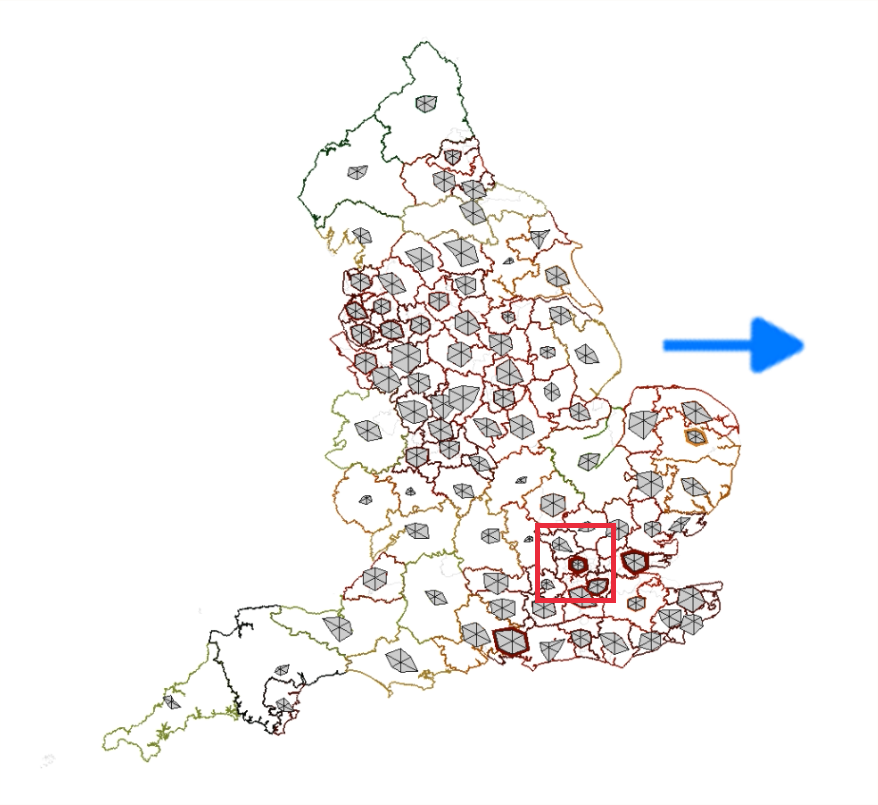
\includegraphics[width=0.48\linewidth]{images/ch5/london01}}
\subfloat{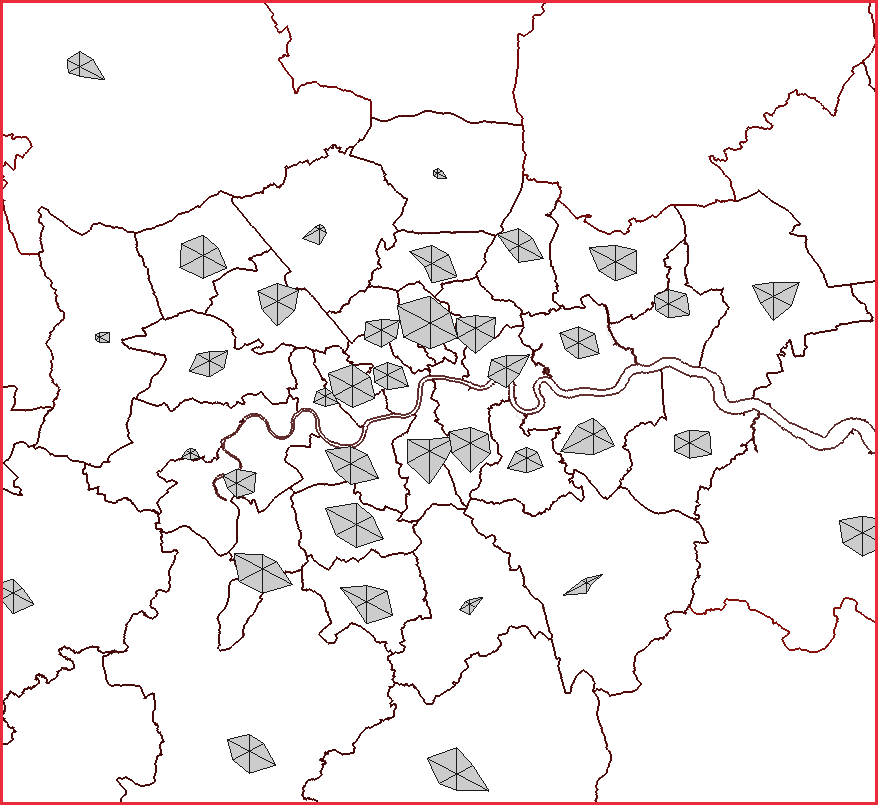
\includegraphics[width=0.48\linewidth]{images/ch5/london02-1}}
\caption{After identifying the southwest of London as having lower prevalence rates than the rest of London (red box), we zoom in to see the cause. We can see low prevalence rates are more frequent among the northwest, with some low prevalence rate in the southeast. We can also now identify the particular CCGs. Glyph scale increased for zoomed in view. See Section \ref{sec:case01}.} \label{fig:case01}
\end{figure}


\subsubsection{Case 2: Counties of the United States} \label{sec:case02} 
Our second example explores counties in the US. We look at the average income over 40 years for each county in the United States from 1979, 1989, 1999, to 2009 in 10 year increments \cite{usCounties}. The US consists of over 3,000 counties.

Rendering the glyphs presents a large frequency of occlusion and therefore we use the estimated minimum size, $m$, to reduce the large number of glyphs to something more accessible.  Starting with the pie chart shows a standard distribution where the average income increases per time period (\textbf{T1} -- overview). Since each glyph represents a number of areas, we adjust the range indicator to represent areas that are rendered, and switch to a polar area chart to visualize the data (Figure \ref{fig:grid}(b)). The wheel glyph shows higher income on the east and west coasts, with the lowest value glyphs across the center of the United States. Wyoming and Montana have some uncommon behavior, where 1979 and 2009 show much stronger average income than their other variants. Zooming in, Wyoming exhibits a tendency to exhibit a higher average income in 1979 over the 40 years, independent of their standing amongst the rest of the US counties. The counties of Sublette and Teton are the exceptions to this which hold stronger mean incomes in 1999 and 2009. See Figure \ref{fig:case02}.


\begin{figure}[t]
\subfloat{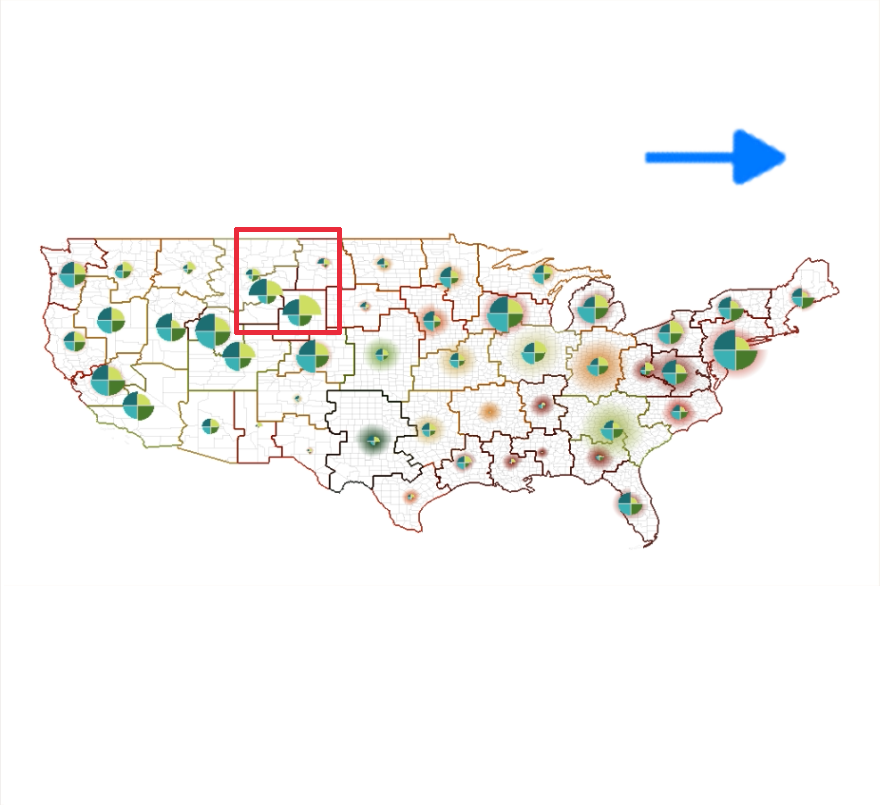
\includegraphics[width=0.48\linewidth]{images/ch5/us01}}
\subfloat{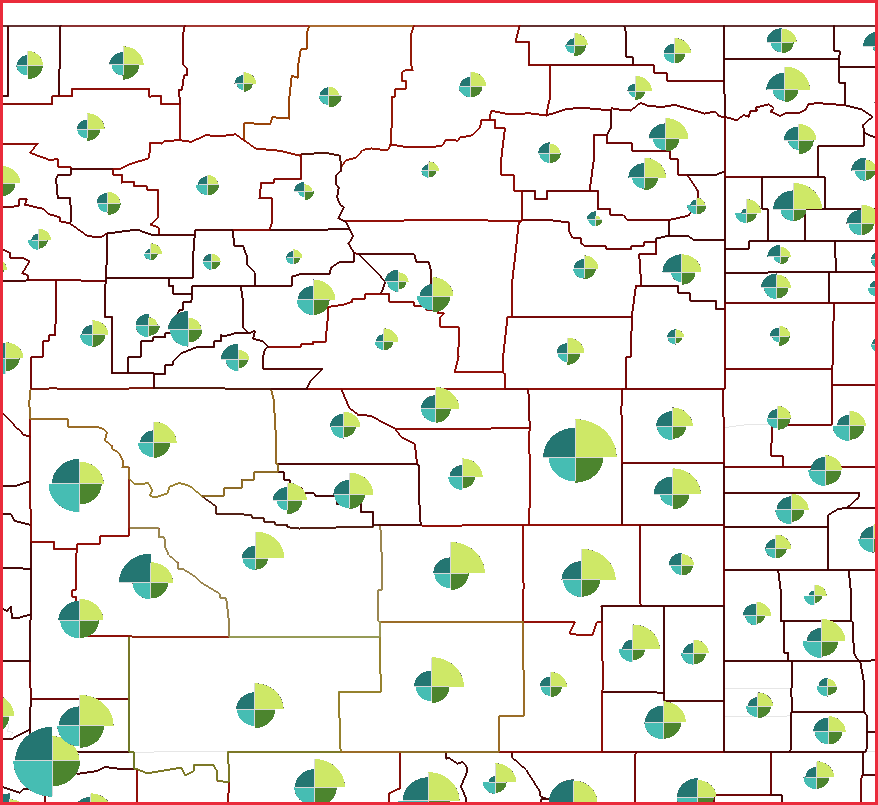
\includegraphics[width=0.48\linewidth]{images/ch5/us02-1}}
\caption{We notice counties around Wyoming and Montana have are higher average income in 1979 and 20019 than usual, We zoom in, and can verify this amongst particular counties. Glyph scale increased for zoomed in view. See Section \ref{sec:case02}.} \label{fig:case02}
\end{figure}
\begin{figure}[t]
\subfloat{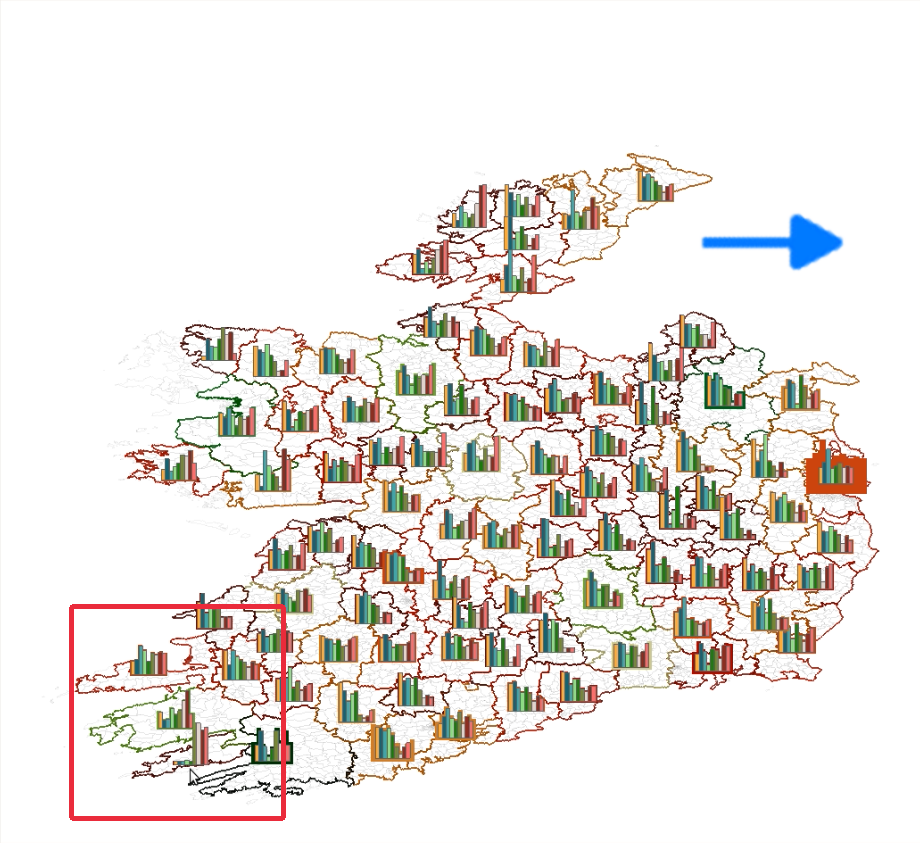
\includegraphics[width=0.48\linewidth]{images/ch5/ireland01}}
\subfloat{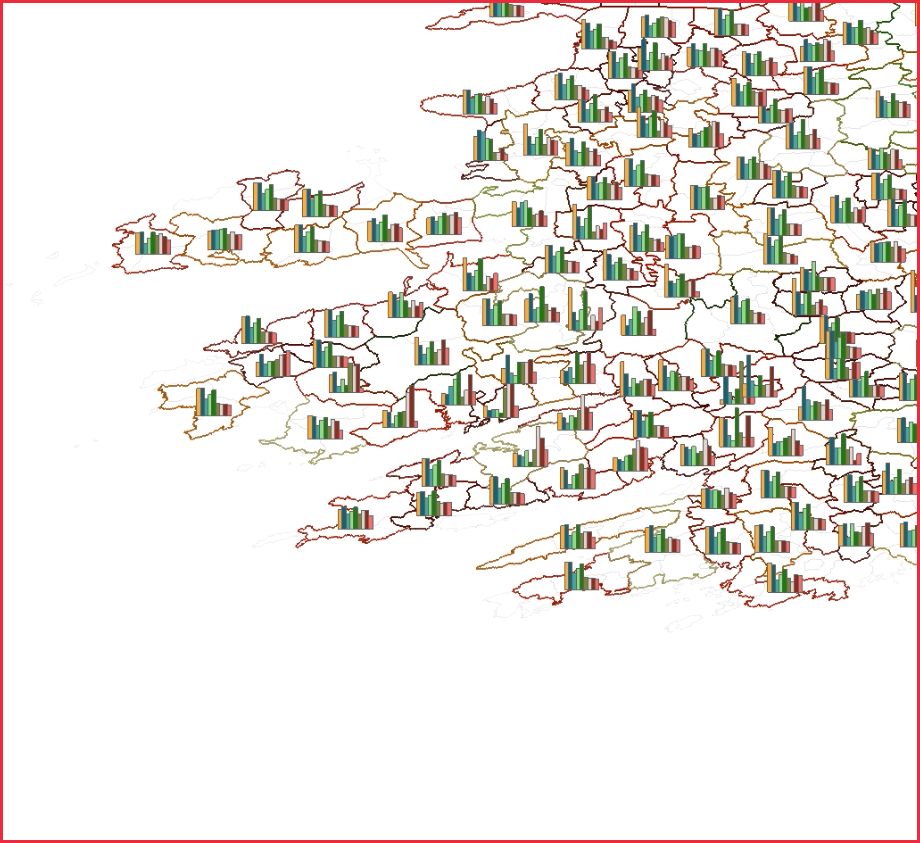
\includegraphics[width=0.48\linewidth]{images/ch5/ireland02}}
\caption{After noticing a strange inconsistency in the south-east of the Republic of Ireland, we zoom in and can verify that this trend can be found amongst a selection electoral divisions. Glyph scale increased for zoomed in view. See Section \ref{sec:case03}.} \label{fig:case03}
\end{figure}
\subsubsection{Case 3: Electoral Divisions of the Republic of Ireland} \label{sec:case03}

For our final case, we look at the electoral divisions of the Republic of Ireland. Our data set looks at population distribution across each division, which is split into nine groups, 0--9 years old, 10--19, 20--29...up to 80+ \cite{electoralDivisions}. There are over 3,400 electoral divisions in the Republic of Ireland.

Similar to Case 2, there are a large number of electoral divisions so we immediately choose to reduce the visible areas to a perceivable number using the estimated scale glyph placement, and adjust a filter to represent a clamped range. In this example, we use bar charts to represent the data. If we look towards Munster, we can see an unusual population distribution, where the proportion of the population, 50 or above, is uncommonly high, and the proportion of people, under 50, is uncommonly low (Figure \ref{fig:f+c}). Zooming in, Glanmore, Canuig, Tahilla, Derriana, Dawros, Ardea, Castlecove, and Caher seem to be the leading factors in this trend. See Figure \ref{fig:case03}.

\begin{figure*} \centering
\subfloat{
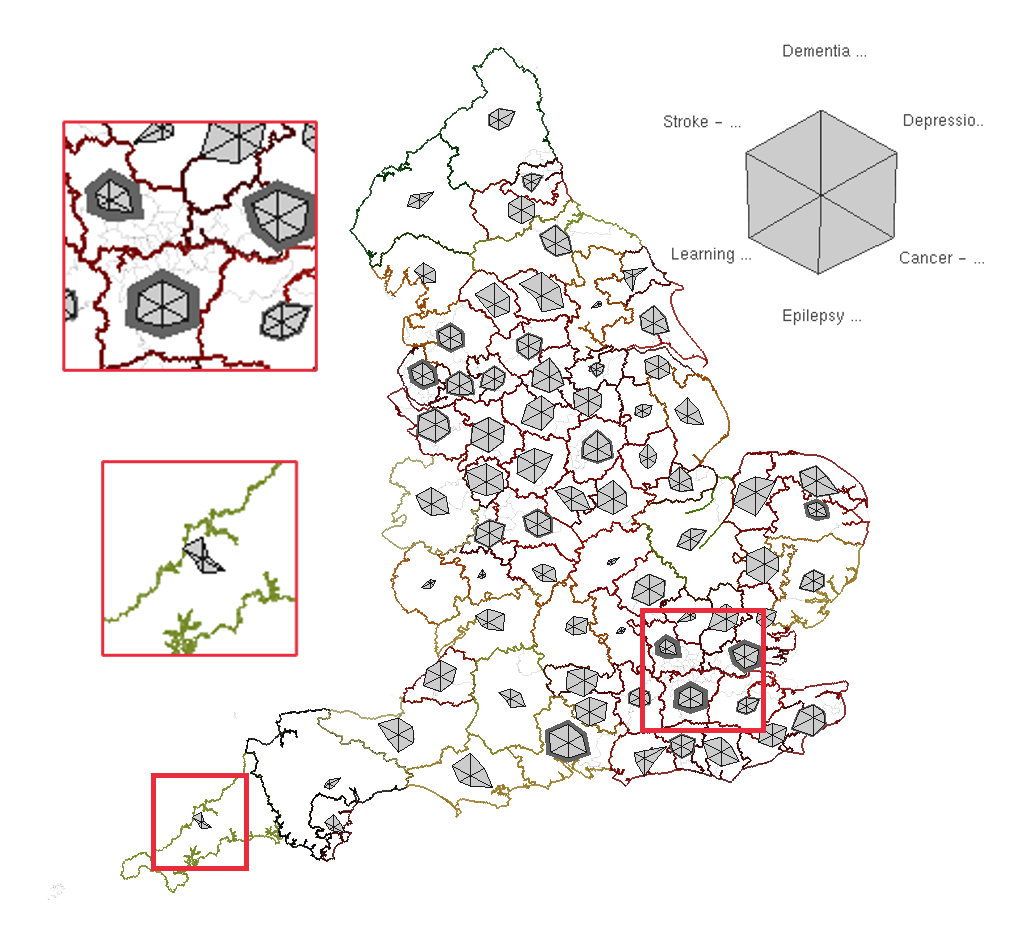
\includegraphics[width=0.32\textwidth]{images/ch5/CCGgridAFull2.png}}
\subfloat{
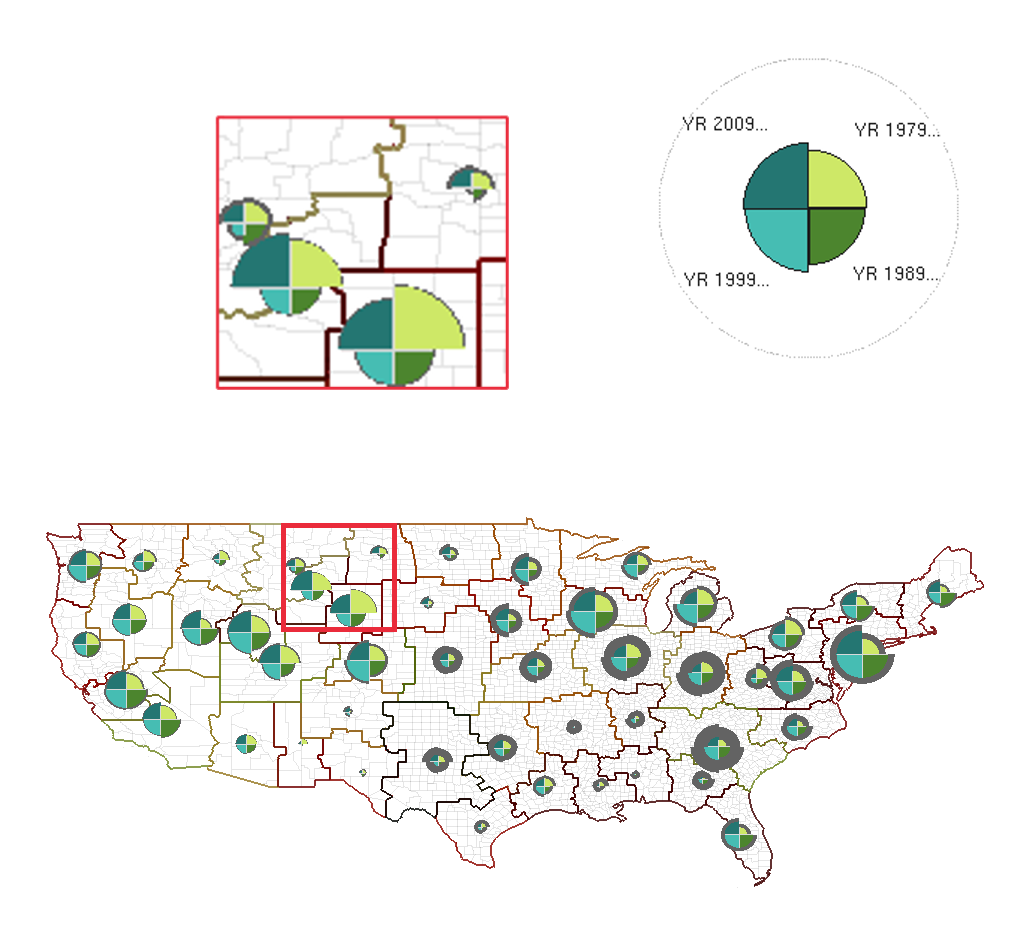
\includegraphics[width=0.32\textwidth]{images/ch5/USgridAFull2.png}}
\subfloat{
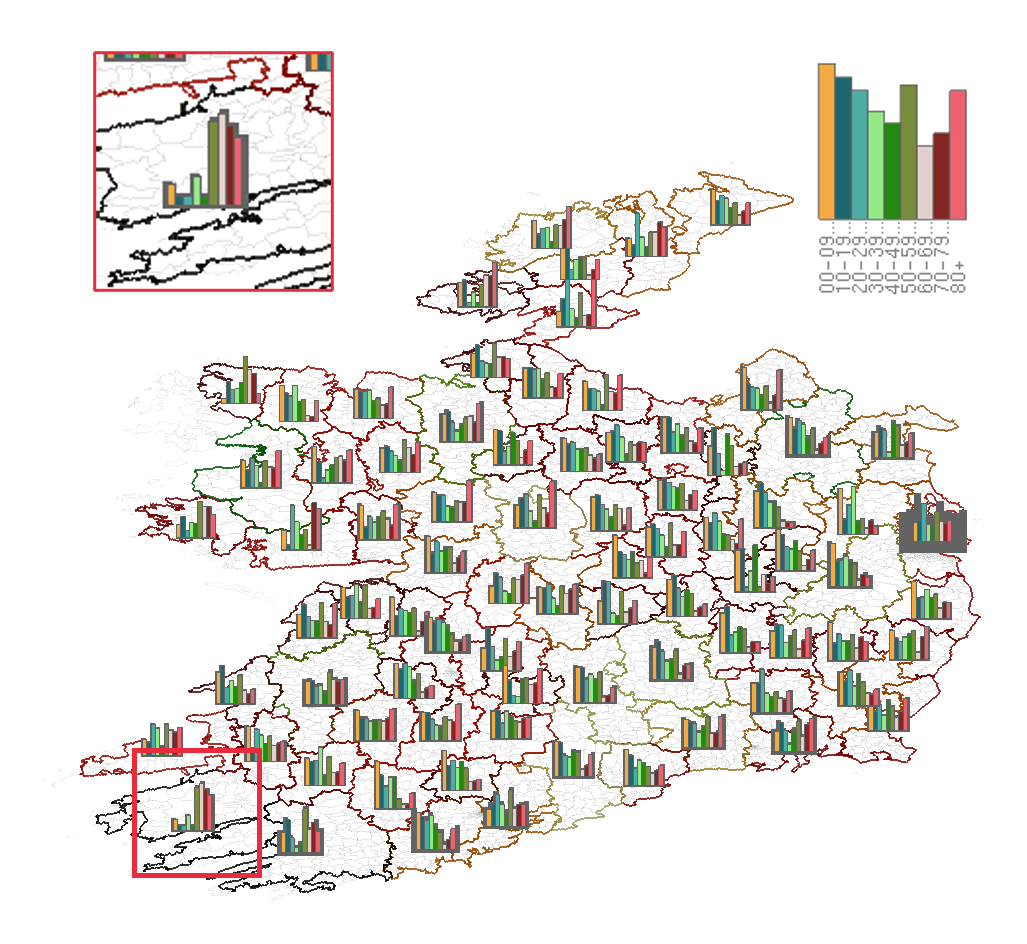
\includegraphics[width=0.32\textwidth]{images/ch5/irelandgridAFull2.png}}
\setcounter{subfigure}{0}
\subfloat[]{
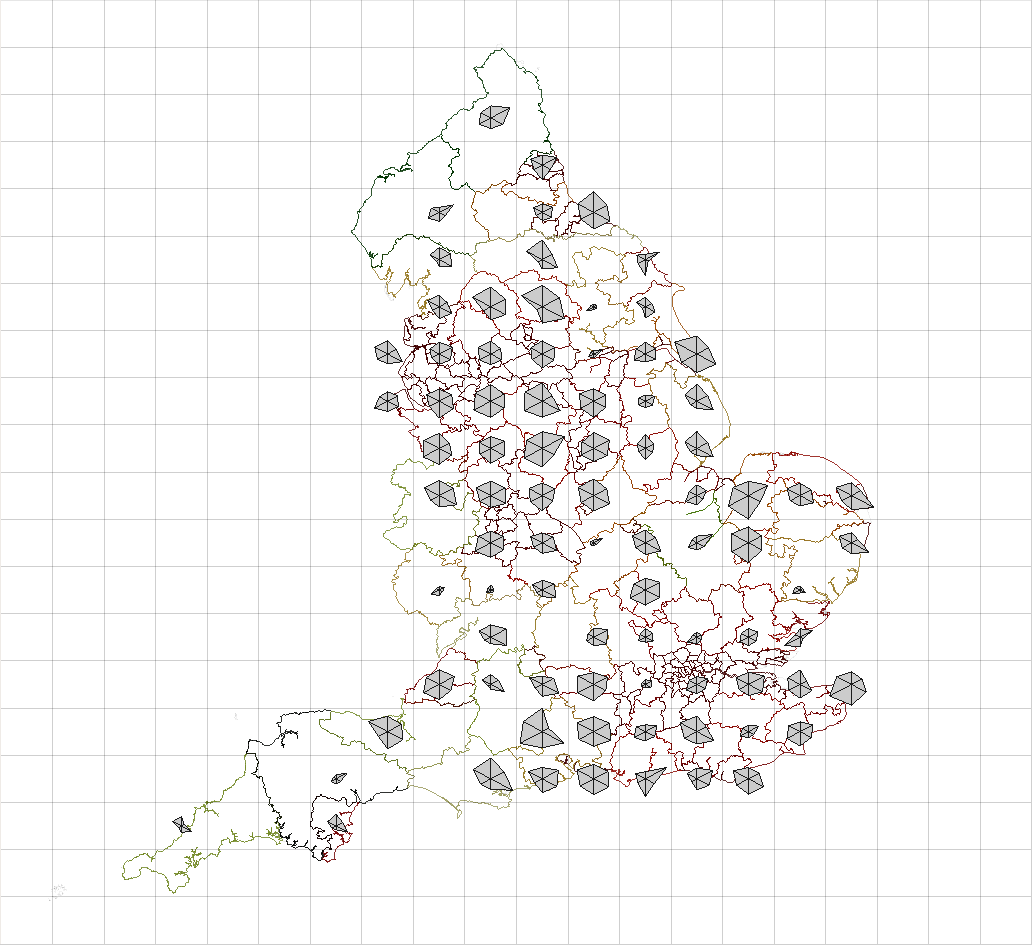
\includegraphics[width=0.32\textwidth]{images/ch5/CCGgridBFull.png}}
\subfloat[]{
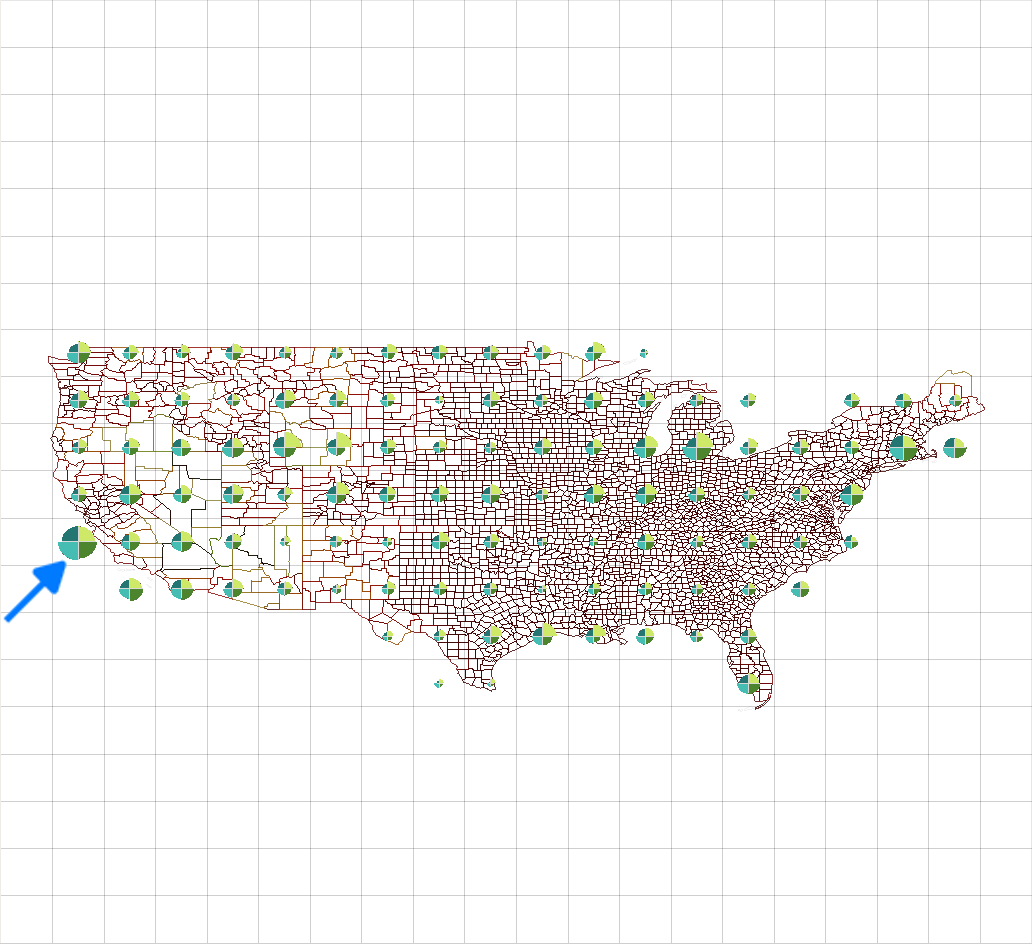
\includegraphics[width=0.32\textwidth]{images/ch5/USgridBFull.png}}
\subfloat[]{
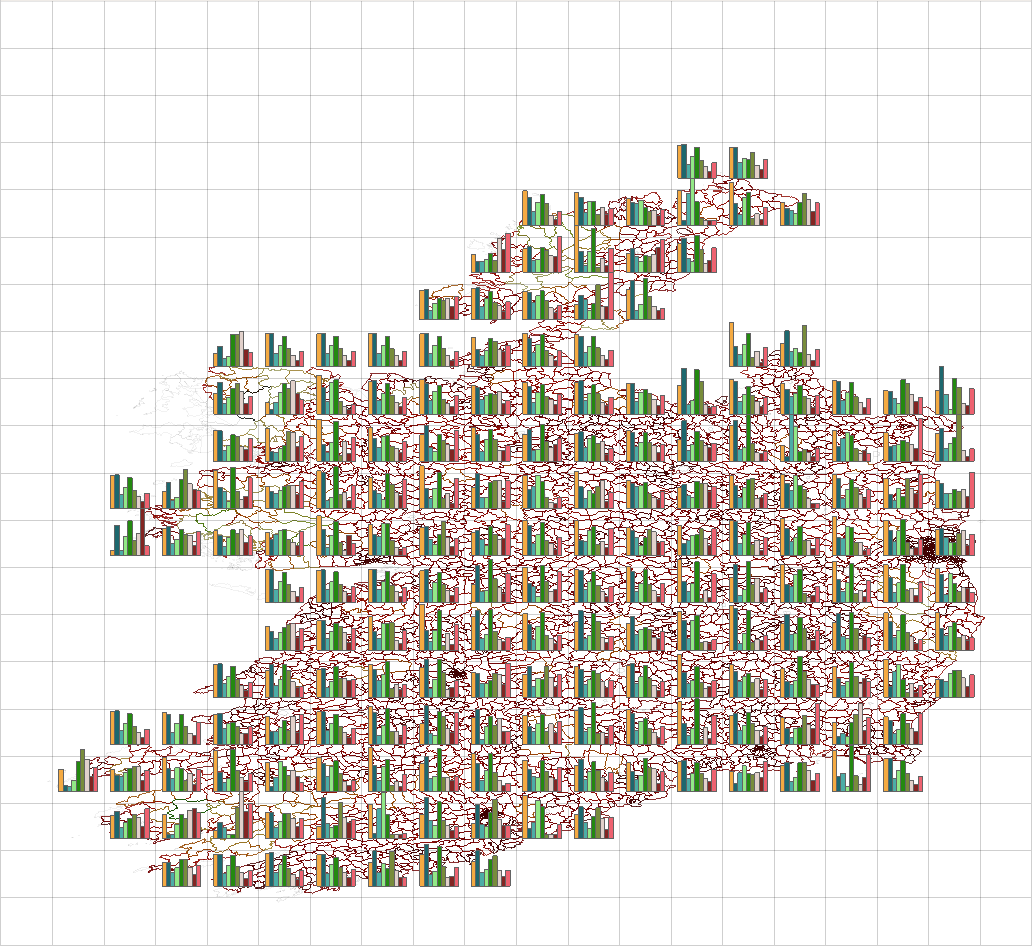
\includegraphics[width=0.32\textwidth]{images/ch5/irelandgridBFull.png}}
\caption{Glyph-placement comparison: top row -- our method, bottom row -- grid-based. (a) Comparison of CCGs (b) Comparison of US Counties (c) Comparison of Ireland's Electoral Divisions. Glyphs based on grid-placement are often de-coupled from the geo-space the represent. The blue arrow signifies the cause of the incomparable data values. See Section \ref{sec:grid}. } \label{fig:compare} \label{fig:grid}
\end{figure*}
\subsection{Comparative Evaluation: Grid-Placement vs. Dynamic Placement} \label{sec:grid}
We evaluate user interpretation of the data against a typical grid structure for glyph placement. We use a Cartesian grid (20$^2$) structure that places glyphs at approximately the same size and resolution as our presented process. Each area is assigned to a cell of the grid, closest to its centroid, where glyphs are derived using the same process as our algorithm. In terms of design, we try to keep both structures similar. In our algorithm, we use a thickened outline to signify the unified area the glyph presents which is not possible for the grid placement version because unit areas are arbitrarily split using a Cartesian grid. We therefore show the presented areas using a lower line width to avoid over representation. Other than this, all design elements are the same and we allow the user to adopt filters and user options identically. However, we use a standard grid structure and therefore the grid structure does not necessarily handle multiple levels of detail. Examples are shown in Figure \ref{fig:grid}.

We look at two main aspects of placement, geo-metric coupling, and value representation. First we examine geo-metric coupling. As the grid is uniform, in all instances, the grid allows for a larger number of glyphs, however, this can be seen as a clear positive. If we start with Figure \ref{fig:grid}(a), it is sometimes difficult to verify where a glyph is when areas reside within a corner of multiple grid slots. If we look at the central-east coast of England, identifying even large areas becomes difficult. This is because the areas are considered uniform, and therefore are distorted uniformly, as opposes to our presented algorithm which attempts to avoid this as much as possible.  In examples Figure \ref{fig:grid}(b), our placement uses fewer glyphs due to the large variance in wheel glyph extents, as opposed to the grid placement that presents roughly twice as many. The grid results in the same limitation as above, with a strong difficulty in understanding how values are mapped to their glyph counterparts. We run into a second problem with the density of the areas, where administrative areas make it difficult to perceive where a grid cell covers, providing little understanding of the context. Both of these problems follow on to Figure \ref{fig:grid}(c).

For value representation, the algorithms do show differences, which is to be expected, in accordance with the modifiable areal unit problem \cite{openshaw1984modifiable}. For Figure \ref{fig:grid}(a), both representations pointed to the same observation in our case study. Figure \ref{fig:grid}(b), exhibits a significant difference. The grid-placement greatly skews the value representation of the US counties, due to some grid elements covering secluded cells. The west coast contains a grid cell with San Francisco, which causes most of the other glyphs to be quite small, independent of the data range option selected. It becomes difficult to compare the two placement options. Although that is the case, both placement schemes lead to the observation found that the time period of 1979 maps to a larger segment in Wyoming. Figure \ref{fig:grid}(c) also  presents the observations found in our case study, although the concentration is more spread out, which can be considered better for examinations. If we consider the ability to zoom, we feel that only the Cartesian grid representation of the Republic of Ireland can lead to a fair comparison for observation, and this is only based on trial-and-error.

%\section{Future Work}
%There are many avenues for future work we can consider. At the moment, we use the raw derived centroid as a placement strategy. although this removes a lot of density and occlusion, there is still some wasted space. We believe that by adding some overlap removal, we could use space more efficiently, whilst still avoiding any decoupling problems. Although we present some case studies, the algorithm could be more carefully compared to other glyph placement strategies with a user-study evaluation. Although we think the use of transitions was a great tool for understanding variation, it is not always necessary. We feel that there are many avenues for exploring at multiple levels of detail. For example, directly zooming to a glyphs unit area extents may not need to represent zooming, to speed up exploration.
\section{Conclusion}
We present a glyph placement algorithm supporting multivariate geospatial visualization at different levels of detail.  We discuss how we create scale aware map, and apply the process to glyph placement. We also discuss the different glyph options and filters we have designed to support exploration of multivariate data. Finally, we review the algorithm by examining the separate use cases, and compare against a pre-existing glyph placement strategy.
%\begin{figure}[t]
%\centering
%\subfigure[]{
%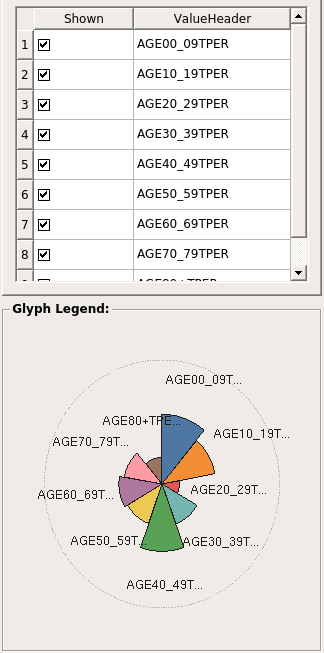
\includegraphics[width=0.6\linewidth]{images/GlyphLegendAndFilter.png}}
%\caption{.} \label{fig:uahindicator}
%\end{figure}


%\section{Acknowledgments}
%We would like to thank KESS for contributing funding towards this endeavor. Knowledge Economy Skills Scholarships (KESS) is a pan-Wales higher level skills initiative led by Bangor University on behalf of the HE sector in Wales. It is partially funded by the Welsh Government's European Social Fund (ESF) convergence programme for West Wales and the Valleys. We would also like to thank XX and XX for help with proofreading the paper.

%-------------------------------------------------------------------------

%\bibliography{references}
%\clearpage
%%-------------------------------------------------------------------------
\begin{figure*} \centering
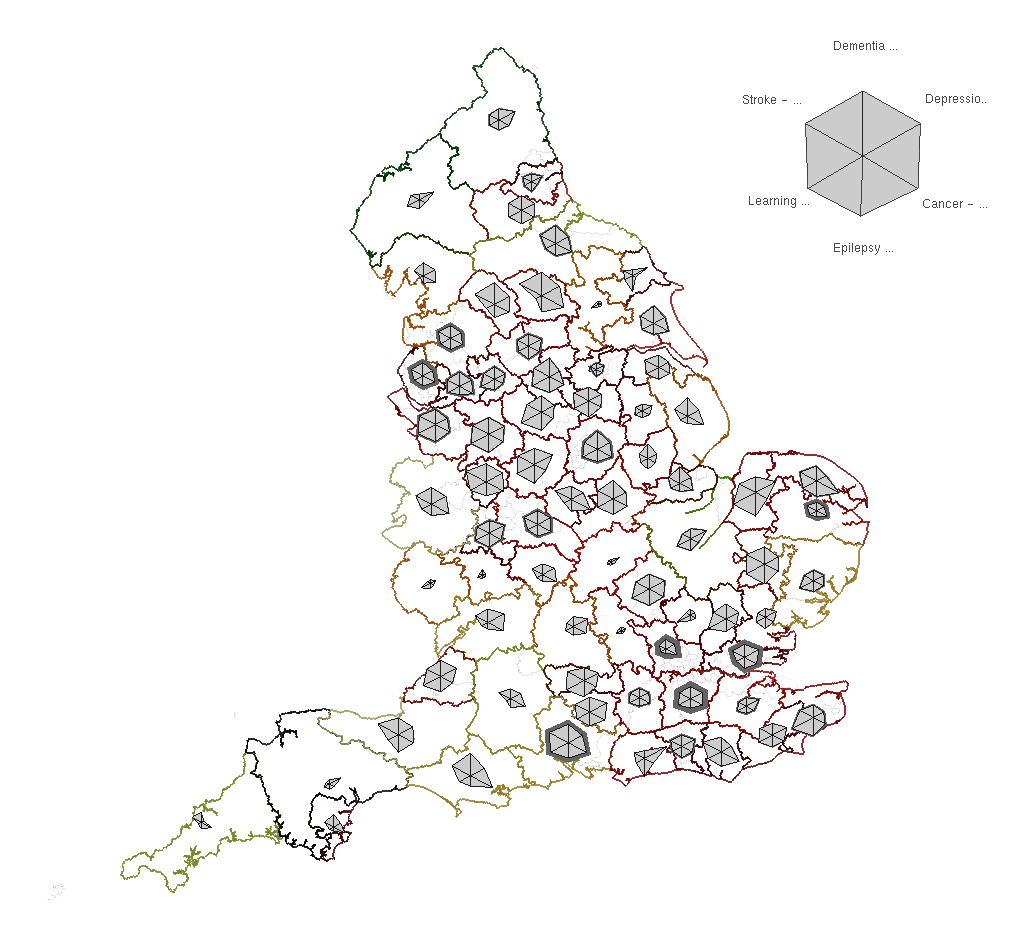
\includegraphics[width=1\textwidth]{images/ch5/CCGgridAFull.png}
\caption{Standard representation of the glyph placement algorithm using the CCGs of England \cite{publicHealthEngland}, with star glyphs. The glyph represents the prevalence of afflictions per CCG area. The legend represents the average prevalence across all glyphs. } \label{fig:sample1}
\end{figure*}
\begin{figure*} \centering
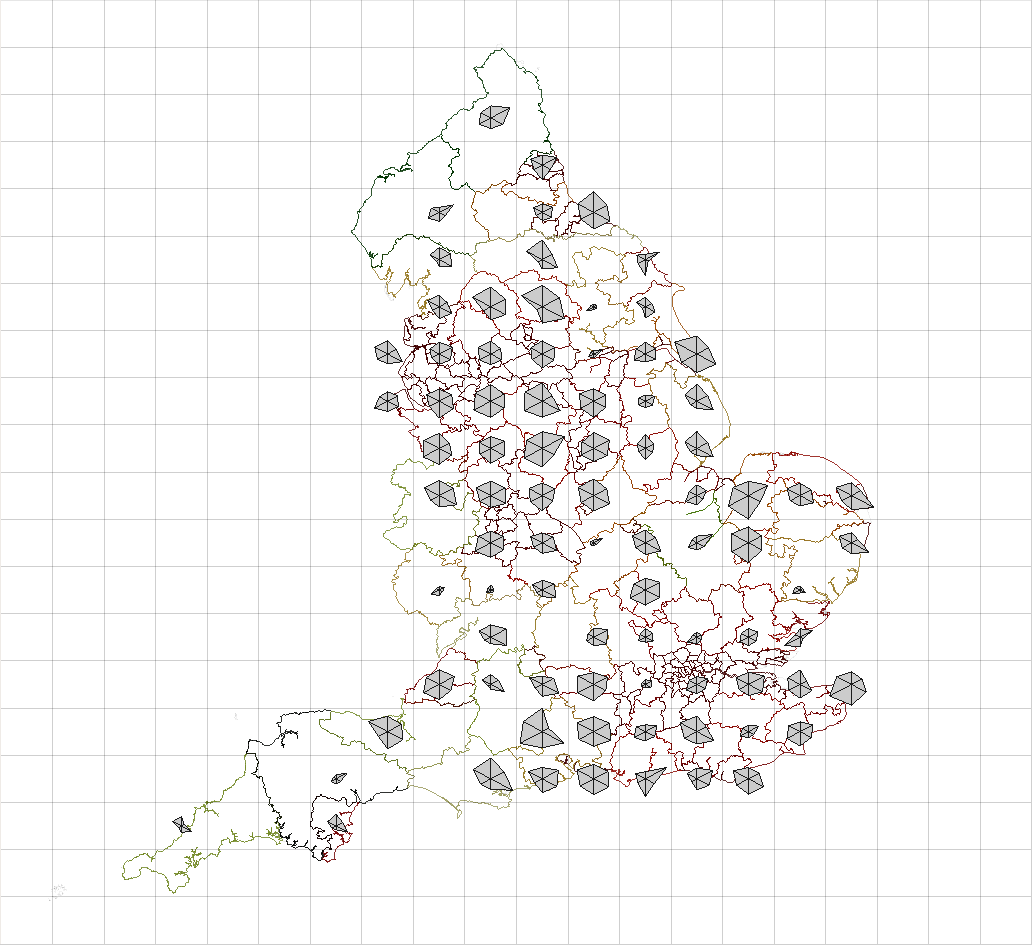
\includegraphics[width=1\textwidth]{images/ch5/CCGgridBFull.png}
\caption{A comparison piece for our CCG sample in Figure \ref{fig:sample1}. The grid-placement is a $20^2$ grid and assigns values in a similar fashion to our concept.}
\end{figure*}
\begin{figure*} \centering
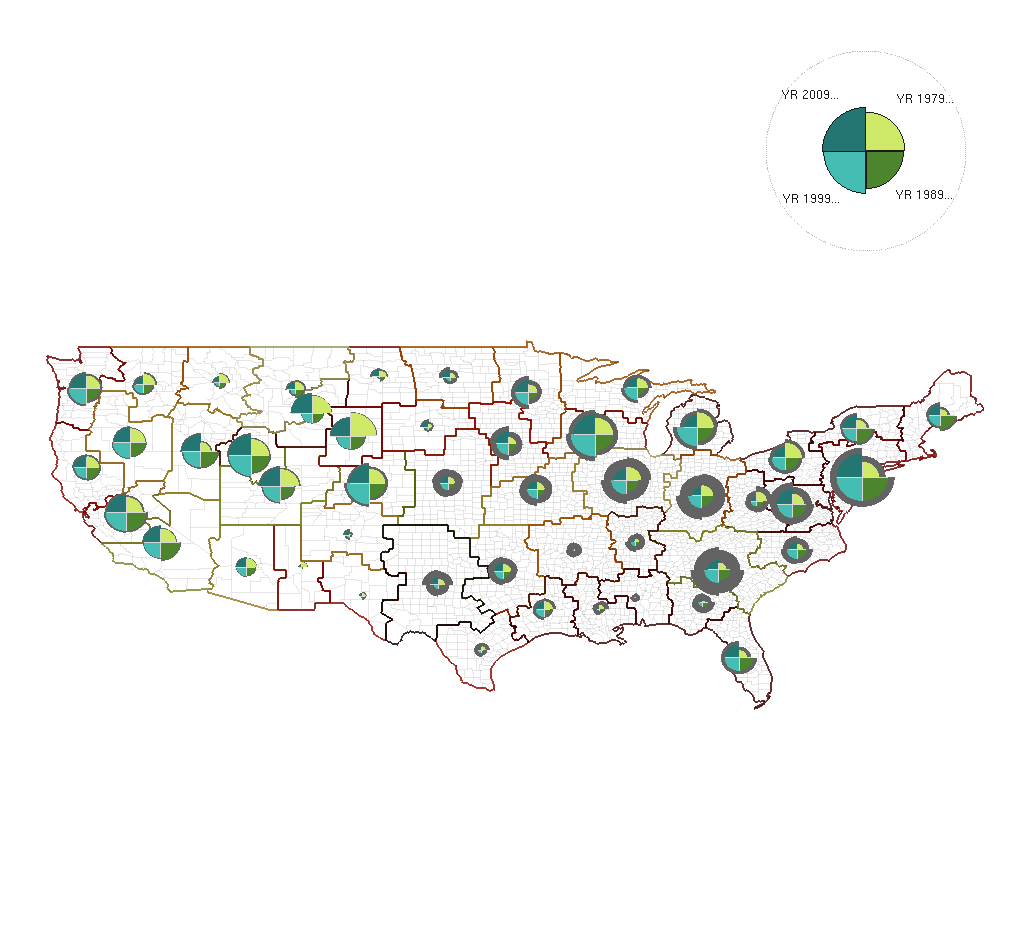
\includegraphics[width=1\textwidth]{images/ch5/USgridAFull.png}
\caption{Standard representation of the glyph placement algorithm using counties of mainline United States. \cite{usCounties}, with polar area glyphs. The glyph represents the average income per household over four time periods, 1979, 1989, 1999, and 2009. The legend represents the average income across all glyphs. } \label{fig:sample2}
\end{figure*}
\begin{figure*} \centering
\includegraphics[width=1\textwidth]{images/ch5/USgridBFull2.png}
\caption{A comparison piece for our US counties sample in Figure \ref{fig:sample2}. The grid-placement is a $20^2$ grid and assigns values in a similar fashion to our concept.}
\end{figure*}
\begin{figure*} \centering
\includegraphics[width=1\textwidth]{images/ch5/irelandgridAFull.png}
\caption{Standard representation of the glyph placement algorithm using electoral divisions of the Republic of Ireland. \cite{electoralDivisions}, with bar glyphs. The glyph represents the age distribution per electoral division in 10 year increments up to 80. The legend represents the average age representation across all glyphs. } \label{fig:sample3}
\end{figure*}
\begin{figure*} \centering
\includegraphics[width=1\textwidth]{images/ch5/irelandgridBFull.png}
\caption{A comparison piece for our electoral divisions sample in Figure \ref{fig:sample3}. The grid-placement is a $20^2$ grid and assigns values in a similar fashion to our concept.}
\end{figure*}
%%\begin{figure*}
%%\centering
%%\subfloat{
%%\includegraphics[width=0.18\linewidth]{images/transition/01.png}}
%%\subfloat{
%%\includegraphics[width=0.18\linewidth]{images/transition/02.png}}
%%\subfloat{
%%\includegraphics[width=0.18\linewidth]{images/transition/03.png}}
%%\subfloat{
%%\includegraphics[width=0.18\linewidth]{images/transition/04.png}}
%%\subfloat{
%%\includegraphics[width=0.18\linewidth]{images/transition/05.png}}\\
%%\subfloat{\includegraphics[width=0.12\linewidth]{images/transition/11}}
%%\subfloat{\includegraphics[width=0.12\linewidth]{images/transition/12}}
%%\subfloat{\includegraphics[width=0.12\linewidth]{images/transition/13}}
%%\subfloat{\includegraphics[width=0.12\linewidth]{images/transition/14}}
%%\subfloat{\includegraphics[width=0.12\linewidth]{images/transition/15}}
%%\subfloat{\includegraphics[width=0.12\linewidth]{images/transition/16}}
%%\subfloat{\includegraphics[width=0.12\linewidth]{images/transition/17}}
%%\caption{An example of a smooth transition made between two child glyphs. Both child glyphs decrease in opacity, whilst the new parent glyph increases in opacity. Refer to Section \ref{sec:transitions}.} \label{fig:grid}
%%\end{figure*}
%%\begin{figure}[t]
%%\centering
%%\subfigure[]{
%%\includegraphics[width=0.08\textwidth]{images/outline0.png}}
%%\subfigure[]{
%%\includegraphics[width=0.08\textwidth]{images/outline1.png}}
%%\subfigure[]{
%%\includegraphics[width=0.08\textwidth]{images/outline2.png}}
%%\subfigure[]{
%%\includegraphics[width=0.08\textwidth]{images/outline3.png}}
%%\subfigure[]{
%%\includegraphics[width=0.08\textwidth]{images/outline4.png}}
%%\caption{ The different types of unit area quantity indicators. (a) No indicator. (b) Outline. (c) Size. (d) Size+Outline. (e) Shadow.} \label{fig:uahindicator}
%%\end{figure}
%%\begin{figure}[t]
%%\centering
%%\subfigure[]{
%%\includegraphics[width=0.08\textwidth]{images/pie.png}}~~~~
%%\subfigure[]{
%%\includegraphics[width=0.08\textwidth]{images/polarareachart.png}}~~~~
%%\subfigure[]{
%%\includegraphics[width=0.08\textwidth]{images/bar.png}}~~~~
%%\subfigure[]{
%%\includegraphics[width=0.05\textwidth]{images/star.png}}~~~~
%%\caption{(a) Pie Chart (b) Polar Area Chart (c) Bar Chart (d) Star Chart. Each glyph represents the same data attributes.} \label{fig:glyphs}
%%\end{figure}
%\begin{figure*}[b]
%\centering
%\subfigure[]{\includegraphics[width=0.48\linewidth]{images/belowAverageFilter.png}}
%\subfigure[]{\includegraphics[width=0.48\linewidth]{images/aboveAverageFilter.png}}
%\caption{(a) Below Average Query Filter. (b) Above Average Query Filter. Refer to Section \ref{sec:filter}.} \label{fig:advancedfilter}  \vspace{-0.2cm}
%\end{figure*}
%
%\begin{figure*}[b]
%\centering
%\subfloat{\includegraphics[width=0.48\linewidth]{images/leafPerDimension.png}}
%\subfloat{\includegraphics[width=0.48\linewidth]{images/clampedPerDimension.png}}\\
%\subfloat{\includegraphics[width=0.48\linewidth]{images/leafOverall.png}}
%\subfloat{\includegraphics[width=0.48\linewidth]{images/clampedOverall.png}}\\
%\caption{Data Range Options. Refer to Section \ref{sec:filter}.} \label{fig:clamp}  \vspace{-0.2cm}
%\end{figure*}


